%% =====================================================================================
%% 1 Introduction. Spine of the paper, three sentences:
%%   believed: LLM agents that reach cooperative outcomes are cooperating strategically;
%%   found:    when the prompt leaves the agent's goal unstated, the models pay by default
%%             (play that does not follow the stakes, visible where paying cannot help);
%%             removing normative words keeps the default, stating the goal switches most
%%             of it off without making the models weigh the risk; defaults respond to
%%             partners only in simple ways and fail predictably in mixed groups and under
%%             selection;
%%   change:   state the agent's goal, evaluate against the optimum, in mixed populations,
%%             and choose the selection signal with care.
%% Scope rule: claims are about the five low-cost models tested, not about "LLMs".
%% Model names: always with the family (Claude Haiku, Gemini Flash-Lite, GPT Luna, Qwen,
%% Grok); a bare "Luna" does not tell the reader it is a GPT model.
%% =====================================================================================
\section{Introduction}
\label{sec:intro}
%% =====================================================================================
%% Overview figure (figure*, text width). Drawn by analysis/overview.py from the counts in
%% tables/num_selfplay.tex; placed right after \label{sec:intro} so it floats to page 2.
%% =====================================================================================
\begin{figure*}[t]
\centering
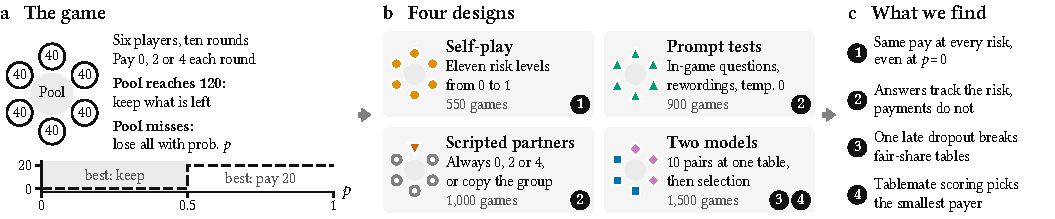
\includegraphics[width=\textwidth]{figures/fig_overview.pdf}
\Description{A three-part overview read from left to right. First, the game: six seats, each
holding 40 units, sit around a shared pool; each round a seat pays 0, 2 or 4, and a small
step plot shows that the best total per seat is 0 below catastrophe probability one half and
20 above it. Second, four design cards, each with a small table of model markers and a game
count: self-play on eleven risk levels, prompt tests, one model beside scripted partners, and
two models at one table followed by selection. Third, four numbered findings that match
numbered badges on the cards.}
\caption{Overview. (a)~Six players hold 40 units and pay 0, 2 or 4 into a shared pool in each
of ten rounds; if the pool misses 120, all savings are lost with probability $p$. Below: the
best total per seat (Proposition~\ref{prop:eq}). (b)~The designs, who sits at each table, and
the number of games. (c)~The findings; badges mark the design behind each.}
\label{fig:overview}
\end{figure*}


Language-model agents are starting to act for people in shared settings: they spend
budgets, share compute, and bargain over common resources. Each such agent is a player in a
social dilemma, because what it pays helps the group and costs its owner. Before deploying
one, a designer needs answers to two questions. Does the agent's cooperation depend on what
is at stake? And does it depend on what the other agents do?

Self-play, the most common test, cannot answer either question. When every seat holds a copy
of the same model, an agent that reasons about the stakes and an agent that repeats a fixed
rule can write the same record of play. Many studies also report whether the group reached
its goal, not how far the agents were from the best they could have done. Yet a group of
agents can reach its goal and still waste most of its money. Finally, a prompt that gives a
group target and a number of rounds implies an equal split, so an agent that repeats that
split looks cooperative on every summary measure.

We study these questions in a classic game from research on climate cooperation, the
collective-risk social dilemma~\cite{milinski2008collective}. Six players pay into a shared
pool over ten rounds, and if the pool misses a target, a catastrophe destroys everyone's
savings with probability $p$. For risk-neutral players, nobody should pay below a pivot
$\popt=\tfrac12$, and above it everyone should pay the \emph{fair share}, the target split
equally, which is half of each player's money. At $p=0$ paying only lowers a player's own
money, so no attitude to risk can explain it.

We call play a \emph{default} when it does not change with what is at stake. The game gives
two sharp tests of a default, because in both paying cannot help: paying at $p=0$, and
paying after the outcome can no longer change. We test five low-cost production models, one
per provider, in \CntGames{} games and four designs: self-play across eleven risk levels;
prompt controls, including questions about which choice pays more and prompts that remove
normative words or state the agent's goal; one model against five scripted partners, where
the best response can be computed exactly; and two different models at one table, which lets
us ask which agent would win if agents were selected by
payoff~\cite{wellman2006methods,tuyls2018generalised}. Our findings are four
(Figure~\ref{fig:overview}).

\begin{itemize}
\item \textbf{Risk does not change the default} (Section~\ref{sec:risk}). Four models pay
  about the fair share at every positive risk level, and four of five still pay at $p=0$.
  Removing the normative words from the prompt changes neither result. Stating that only
  the agent's own cash matters largely stops three models from paying at $p=0$, but only
  GPT Luna then switches from keeping its money at low risk to paying at high risk. Success
  rates hide the failures that remain.
\item \textbf{Answers track the risk; play does not} (Section~\ref{sec:knowing}). In
  separate calls, several models rank the two choices correctly and change that ranking with
  the risk, but they pay the same amount. Beside scripted partners who make every payment a
  loss, no model pays nothing, and two models keep paying after the outcome is settled.
\item \textbf{An exact fair share has no slack} (Section~\ref{sec:groups}). One partner
  that stops paying in the last round breaks a table of exact fair-share players, while a
  table that overpays a little absorbs it. Agents pay less when generous partners fill most
  of the table.
\item \textbf{The scoring rule decides who is selected} (Section~\ref{sec:selection}).
  Seats at one table share the pool and the lottery, so the smaller payer always earns more
  there. Scoring agents against their tablemates therefore favours the smallest payer and,
  in our games, lowers group success. Scoring them across separate groups favours the exact
  fair-share player at moderate and high risk.
\end{itemize}

For the models we test, cooperation is a default that follows from what the prompt leaves
unsaid, not a choice that follows from the stakes. A default can work well beside partners
like itself, but it cannot be trusted with shared resources, and the way a system states
its agents' goals and selects its agents can make the problem better or worse.
